% !TeX root = ../../Thesis.tex
\ThesisChapter
  {\ThesisText{Experiments and Evaluation}{Experimente und Evaluation}}
  {ch:evaluation}
  {TODO: Add a brief chapter overview. \\
  This chapter describes the experimental setup, metrics, and data analysis and presents the results in a reproducible manner.}

% TODO: Describe the experiments and present their results.

This chapter reports how the solution was evaluated and what was measured.
It presents results; it does not interpret them.

Possible contents include:
\begin{itemize}
  \item the experimental setup and test environment,
  \item the datasets, workloads, scenarios, or test cases used,
  \item the selected metrics and evaluation criteria,
  \item the procedure used to conduct the experiments, including how often each was repeated, and
  \item the obtained results.
\end{itemize}

Describe the setup in enough detail that a reader could repeat the experiments and obtain the same numbers.
Use tables, figures, and diagrams where they help to communicate the findings.

Keep interpretation out of this chapter.
Explaining what the numbers mean, why they differ from expectations, and how they compare with other approaches is the task of the discussion chapter.

The implementation chapter describes how the solution was realized.
This chapter describes how the implemented solution was examined.

% Example for adding a table stored in the chapter-specific table folder.
\section{\ThesisText{Example Result Presentation}{Beispiel: Ergebnisdarstellung}}
\label{sec:example-result-presentation}
\subsection{\ThesisText{Tabular Results}{Tabellarische Ergebnisse}}
\label{sec:tabular-results}

Table~\ref{tab:example-results} shows one possible presentation of scaling measurements.
Numbers and units are set with siunitx, so a runtime of \qty{120.0}{\second} and a bandwidth of \qty{2.4}{\giga\byte\per\second} are formatted identically throughout the document.
% !TeX root = ../../Thesis.tex
\begin{table}[htbp]
  \centering
  \small
  \renewcommand{\arraystretch}{1.25}
  \setlength{\tabcolsep}{12pt}
  % The S columns come from siunitx and align the numbers on the decimal marker.
  % Header cells must be braced so that siunitx does not try to parse them as numbers.
  \begin{tabular}{r S[table-format=3.1] S[table-format=1.2] S[table-format=3.1]}
    \toprule
    {\textbf{\ThesisText{Compute nodes}{Rechenknoten}}} &
    {\textbf{\ThesisText{Runtime}{Laufzeit}\ (\unit{\second})}} &
    {\textbf{Speedup}} &
    {\textbf{\ThesisText{Efficiency}{Effizienz}\ (\unit{\percent})}} \\
    \midrule
    1 & 120.0 & 1.00 & 100.0 \\
    2 & 66.7  & 1.80 & 90.0  \\
    4 & 37.5  & 3.20 & 80.0  \\
    8 & 23.5  & 5.11 & 63.9  \\
    \bottomrule
  \end{tabular}
  \caption{\ThesisText{Example scaling results for an illustrative workload.}{Beispielhafte Skalierungsergebnisse für eine illustrative Anwendung.}}
  \label{tab:example-results}
\end{table}


% Example for adding a diagram stored in the chapter-specific figure folder.
\subsection{\ThesisText{Performance Plot}{Leistungsdiagramm}}
\label{sec:performance-plot}

Figure~\ref{fig:example-scaling} visualizes the same measurements and compares them with ideal scaling.
\Cref{tab:example-results} and~\Cref{fig:example-scaling} thus present the same data in two forms.
Unlike \verb|\ref|, \verb|\cref| prints the word \enquote{Table} or \enquote{Figure} itself, so a float that later changes type does not leave a wrong word behind in the running text.

\textbf{Hint:} Whenever suitable, use gnuplot to create plots:~\url{https://www.gnuplot.info/}

\textbf{Important:} Every figure generated entirely or partially using an AI-based tool must be explicitly identified and properly referenced.
The use of AI must be clearly disclosed in the corresponding figure caption.

\begin{figure}[htbp]
  \centering
  % \resizebox also scales the plot's labels; when the label size must match the document font exactly, set the size in the .gp file instead.
  \resizebox{0.75\textwidth}{!}{% GNUPLOT: LaTeX picture with Postscript
\begingroup
  \makeatletter
  \providecommand\color[2][]{%
    \GenericError{(gnuplot) \space\space\space\@spaces}{%
      Package color not loaded in conjunction with
      terminal option `colourtext'%
    }{See the gnuplot documentation for explanation.%
    }{Either use 'blacktext' in gnuplot or load the package
      color.sty in LaTeX.}%
    \renewcommand\color[2][]{}%
  }%
  \providecommand\includegraphics[2][]{%
    \GenericError{(gnuplot) \space\space\space\@spaces}{%
      Package graphicx or graphics not loaded%
    }{See the gnuplot documentation for explanation.%
    }{The gnuplot epslatex terminal needs graphicx.sty or graphics.sty.}%
    \renewcommand\includegraphics[2][]{}%
  }%
  \providecommand\rotatebox[2]{#2}%
  \@ifundefined{ifGPcolor}{%
    \newif\ifGPcolor
    \GPcolortrue
  }{}%
  \@ifundefined{ifGPblacktext}{%
    \newif\ifGPblacktext
    \GPblacktexttrue
  }{}%
  % define a \g@addto@macro without @ in the name:
  \let\gplgaddtomacro\g@addto@macro
  % define empty templates for all commands taking text:
  \gdef\gplbacktext{}%
  \gdef\gplfronttext{}%
  \makeatother
  \ifGPblacktext
    % no textcolor at all
    \def\colorrgb#1{}%
    \def\colorgray#1{}%
  \else
    % gray or color?
    \ifGPcolor
      \def\colorrgb#1{\color[rgb]{#1}}%
      \def\colorgray#1{\color[gray]{#1}}%
      \expandafter\def\csname LTw\endcsname{\color{white}}%
      \expandafter\def\csname LTb\endcsname{\color{black}}%
      \expandafter\def\csname LTa\endcsname{\color{black}}%
      \expandafter\def\csname LT0\endcsname{\color[rgb]{1,0,0}}%
      \expandafter\def\csname LT1\endcsname{\color[rgb]{0,1,0}}%
      \expandafter\def\csname LT2\endcsname{\color[rgb]{0,0,1}}%
      \expandafter\def\csname LT3\endcsname{\color[rgb]{1,0,1}}%
      \expandafter\def\csname LT4\endcsname{\color[rgb]{0,1,1}}%
      \expandafter\def\csname LT5\endcsname{\color[rgb]{1,1,0}}%
      \expandafter\def\csname LT6\endcsname{\color[rgb]{0,0,0}}%
      \expandafter\def\csname LT7\endcsname{\color[rgb]{1,0.3,0}}%
      \expandafter\def\csname LT8\endcsname{\color[rgb]{0.5,0.5,0.5}}%
    \else
      % gray
      \def\colorrgb#1{\color{black}}%
      \def\colorgray#1{\color[gray]{#1}}%
      \expandafter\def\csname LTw\endcsname{\color{white}}%
      \expandafter\def\csname LTb\endcsname{\color{black}}%
      \expandafter\def\csname LTa\endcsname{\color{black}}%
      \expandafter\def\csname LT0\endcsname{\color{black}}%
      \expandafter\def\csname LT1\endcsname{\color{black}}%
      \expandafter\def\csname LT2\endcsname{\color{black}}%
      \expandafter\def\csname LT3\endcsname{\color{black}}%
      \expandafter\def\csname LT4\endcsname{\color{black}}%
      \expandafter\def\csname LT5\endcsname{\color{black}}%
      \expandafter\def\csname LT6\endcsname{\color{black}}%
      \expandafter\def\csname LT7\endcsname{\color{black}}%
      \expandafter\def\csname LT8\endcsname{\color{black}}%
    \fi
  \fi
    \setlength{\unitlength}{0.0500bp}%
    \ifx\gptboxheight\undefined%
      \newlength{\gptboxheight}%
      \newlength{\gptboxwidth}%
      \newsavebox{\gptboxtext}%
    \fi%
    \setlength{\fboxrule}{0.5pt}%
    \setlength{\fboxsep}{1pt}%
    \definecolor{tbcol}{rgb}{1,1,1}%
\begin{picture}(7776.00,4464.00)%
    \gplgaddtomacro\gplbacktext{%
      \csname LTb\endcsname%%
      \put(740,640){\makebox(0,0)[r]{\strut{}$1$}}%
      \csname LTb\endcsname%%
      \put(740,2452){\makebox(0,0)[r]{\strut{}$10$}}%
      \csname LTb\endcsname%%
      \put(740,4263){\makebox(0,0)[r]{\strut{}$100$}}%
      \csname LTb\endcsname%%
      \put(860,440){\makebox(0,0){\strut{}$1$}}%
      \csname LTb\endcsname%%
      \put(1819,440){\makebox(0,0){\strut{}$2$}}%
      \csname LTb\endcsname%%
      \put(2778,440){\makebox(0,0){\strut{}$4$}}%
      \csname LTb\endcsname%%
      \put(3738,440){\makebox(0,0){\strut{}$8$}}%
      \csname LTb\endcsname%%
      \put(4697,440){\makebox(0,0){\strut{}$16$}}%
      \csname LTb\endcsname%%
      \put(5656,440){\makebox(0,0){\strut{}$32$}}%
      \put(6735,640){\makebox(0,0)[l]{\strut{}$1$}}%
      \put(6735,2452){\makebox(0,0)[l]{\strut{}$10$}}%
      \put(6735,4263){\makebox(0,0)[l]{\strut{}$100$}}%
    }%
    \gplgaddtomacro\gplfronttext{%
      \csname LTb\endcsname%%
      \put(2954,4100){\makebox(0,0)[r]{\strut{}±stddev}}%
      \csname LTb\endcsname%%
      \put(2954,3900){\makebox(0,0)[r]{\strut{}mean time}}%
      \csname LTb\endcsname%%
      \put(4817,4100){\makebox(0,0)[r]{\strut{}speedup}}%
      \csname LTb\endcsname%%
      \put(4817,3900){\makebox(0,0)[r]{\strut{}ideal}}%
      \csname LTb\endcsname%%
      \put(190,2451){\rotatebox{-270.00}{\makebox(0,0){\strut{}Mean runtime [s]}}}%
      \put(7315,2451){\rotatebox{-270.00}{\makebox(0,0){\strut{}Speedup  T(1)/T(p)}}}%
      \put(3737,140){\makebox(0,0){\strut{}Nodes}}%
    }%
    \gplbacktext
    \put(0,0){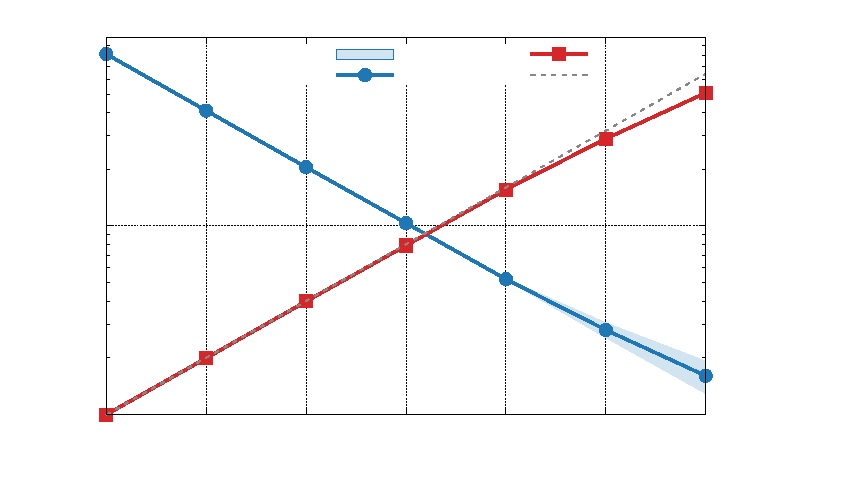
\includegraphics[width={388.80bp},height={223.20bp}]{figures/05/example-scaling-diagram}}%
    \gplfronttext
  \end{picture}%
\endgroup
}
  \caption{\ThesisText{Example diagram comparing measured and ideal parallel scaling.}{Beispieldiagramm mit gemessener und idealer paralleler Skalierung.}}
  \label{fig:example-scaling}
\end{figure}

% Example for adding source code stored in the chapter-specific listing folder.
\subsection{\ThesisText{Source-Code Listing}{Quelltextauszug}}
\label{sec:source-code-listing}
Listing~\ref{lst:example-parallel-sum} demonstrates how source code can be included from a separate file with syntax highlighting and line numbers.

\lstinputlisting[
  float=htbp,
  language=C,
  caption={\ThesisText{Example OpenMP reduction for summing an array in parallel.}{Beispielhafte OpenMP-Reduktion zur parallelen Summation eines Arrays.}},
  label={lst:example-parallel-sum}
]{listings/05/example-parallel-sum.c}
